\chapter{\IfLanguageName{dutch}{Stand van zaken}{State of the art}}
\label{ch:stand-van-zaken}

% Tip: Begin elk hoofdstuk met een paragraaf inleiding die beschrijft hoe
% dit hoofdstuk past binnen het geheel van de bachelorproef. Geef in het
% bijzonder aan wat de link is met het vorige en volgende hoofdstuk.

% Pas na deze inleidende paragraaf komt de eerste sectiehoofding.

Dit onderzoek richt zich op automatische machine learning platformen. Maar alvorens van start te gaan met de onderliggende technieken is het belangrijk om een goed zicht te hebben op de basis waarop het gebouwd is. Zo worden eerst een aantal belangrijke begrippen en technieken besproken, deze sectie kan overgeslagen worden als deze informatie triviaal is voor de lezer. De automatisatie hiervan wordt onderzocht, welke technieken worden met elkaar gecombineerd en hoe bekom je uiteindelijk resultaten. Het is nodig om de theoretische benadering goed te begrijpen om uiteindelijk te kunnen beslissen als het resultaat van het experiment voldoet aan de normen van een goed werkend model. Tot slot worden de beschikbare cloud platformen besproken en vergeleken met een open source library, AutoKeras, dat gebaseerd is op de populaire neurale netwerklibrary, Keras. 

\section{Inleiding machine learning}
\label{sec:inl-machine-learning}

Deze sectie dient om mensen zonder kennis van machine learning bekend te maken met enkele begrippen en technieken binnen het werkveld. Mensen met enige basiskennis kunnen direct doorgaan naar de volgende sectie.

\subsection{Soorten machine learning}
\label{subsec:soorten-machine-learning}

\begin{figure}
    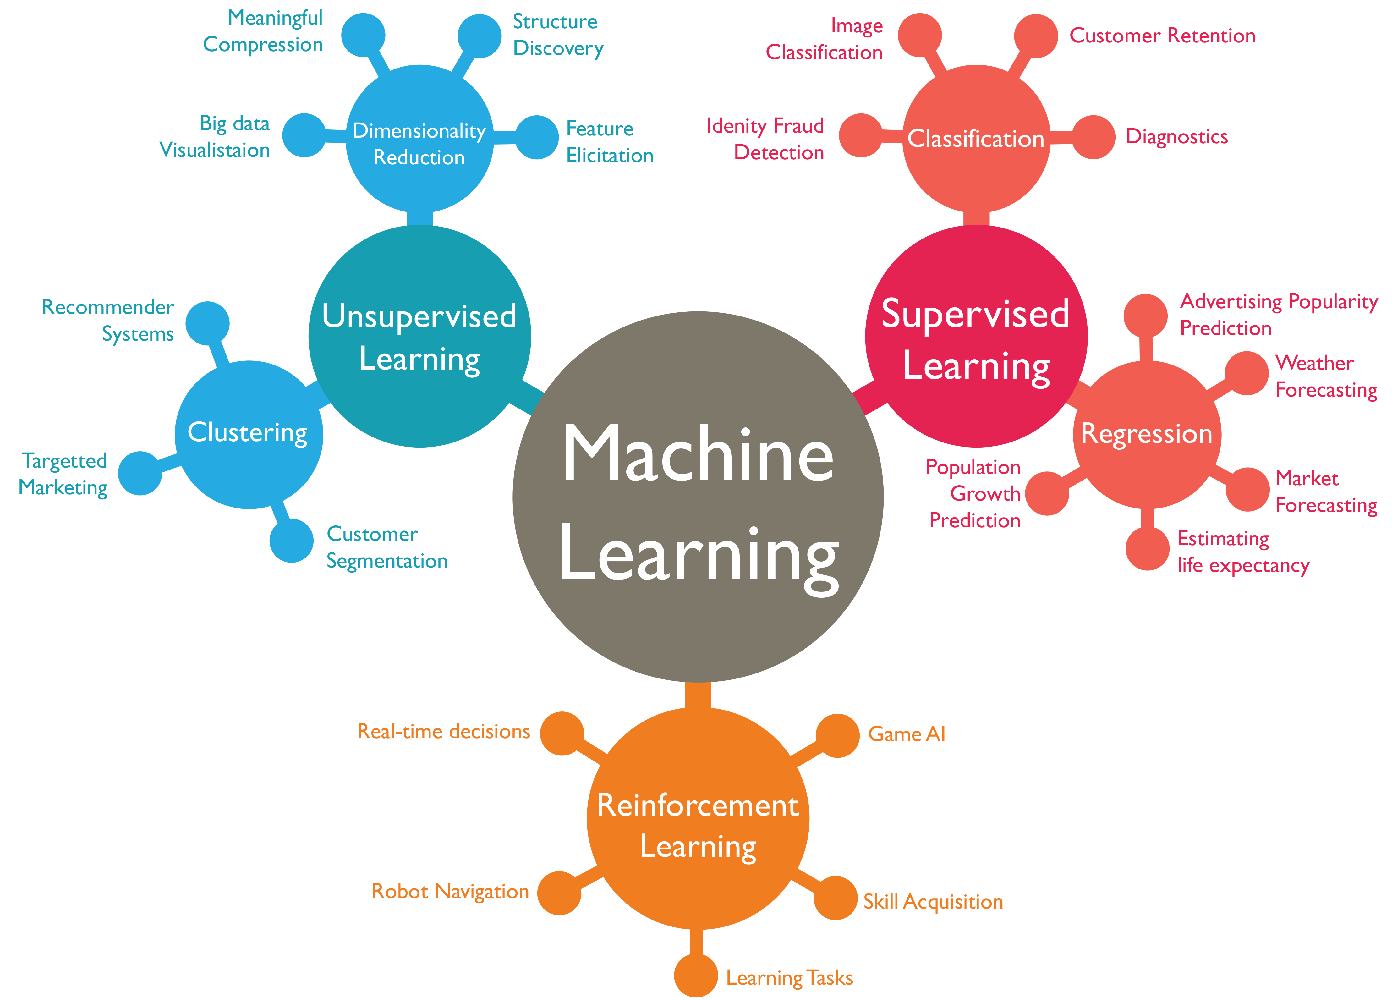
\includegraphics[width=\linewidth]{img/ml-soorten.png}
    \caption{Soorten machine learning met enklele toepassingen. Bron: \url{https://www.linkedin.com/pulse/business-intelligence-its-relationship-big-data-geekstyle}}
    \label{fig:ml-soorten}
\end{figure}

\textcite{Lievens2019} schreef over 3 grote types binnen het domein van machine learning. Deze worden kort verklaard aan de hand van een praktisch voorbeeld. Figuur \ref{fig:ml-soorten} is een algemeen overzicht van wat hieronder beschreven is.


\subsubsection{Gesuperviseerd leren}
\label{subsubsec:gesuperviseerd-leren}

Bij gesuperviseerd leren probeert de software agent een functie te leren die een voorspelling maakt voor een gegeven input. De functie die deze voorspellingen maakt evolueert door het gebruik van een trainingsdataset met input-output waarden \autocite{Norvig1994}.

Classificatie is een typisch probleem dat opgelost wordt met gesuperviseerd leren, het wordt later in dit onderzoek op een andere manier opgelost. Het doel van classificatie is om aan de hand van enkele kenmerken een voorgedefinieerde klasse te voorspellen. Er wordt gesproken van een binair classificatieprobleem als er slechts 2 klassen zijn. Spamdetectie is hier een voorbeeld van. Door de belangrijke woorden uit een bericht te halen wordt er een attribuutvector opgebouwd. Door een model te trainen met duizenden berichten en als ze al dan niet spam zijn, kan het een voorspelling maken voor de gegeven vector \autocite{Lievens2019}.

\subsubsection{Ongesuperviseerd leren}
\label{subsubsec:ongesuperviseerd-leren}

Met ongesuperviseerd leren is het mogelijk om in een ongelabelde dataset patronen te vinden die eerder onbekend waren. Bij elke voospelling wordt voor elke categorie meegegeven hoe zeker het model is over zijn voorspelling \autocite{Hinton1999}.

Een ongelabelde dataset met gegevens over klanten waarvoor je te weten wilt komen als er onderliggende groepen ontdekt kunnen worden. Dit wordt ook clustering genoemd, een mogelijke oplossing is \autocite{Lievens2019}:

\begin{itemize}
    \item Klanten die waarschijnlijk hun contract verlengen.
    \item Ontevreden klanten die bijna zeker hun contract opzeggen.
    \item Klanten die voor een bepaalde aanbieding misschien hun contract verlengen.
\end{itemize}

Deze resultaten worden bekomen door berekeningen uit te voeren op de attribuutvector zonder een outputlabel.

\subsubsection{Reinforcement Learning}
\label{subsubsec:reinforcement-learning}

Reinforcement learning focust zich op de acties die een software agent onderneemt om een zo hoog mogelijke beloning te krijgen. Er is dus geen nood aan een (gelabelde) dataset zoals bij gesuperviseerd en ongesuperviseerd leren. De agent probeert een balans te vinden tussen wat hij weet en wat er kan gebeuren \autocite{Kaelbling1996}. In essentie wil dit zeggen dat de agent probeert te leren welke acties leiden tot de hoogste totale beloning \autocite{Lievens2019}.

Deze techniek wordt verder besproken in het deel over geautomatiseerde machine learning.


Geautomatiseerde machine learning is het automatiseren van het trainingsproces bij een artificieel neuraal netwerk. De lage toegangsdrempel zorgt ervoor dat mensen met beperkte machine learning kennis sneller en simpeler een model kunnen trainen en gebruiken.

\section{Natural Architecture Search}

\begin{figure}
    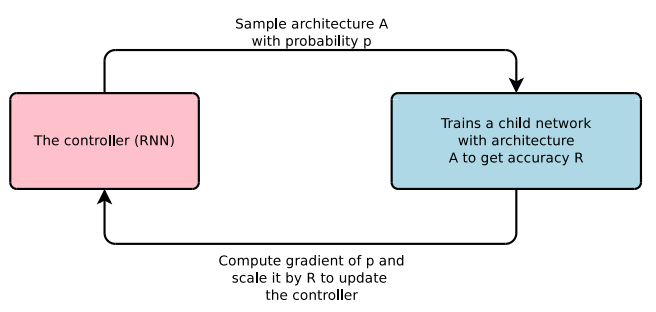
\includegraphics[width=\linewidth]{img/nas.png}
    \caption{Werking van Neural Architecture Search}
    \label{fig:nas-bp}
\end{figure}

Dergelijke AutoML systemen gebruiken een techniek die het ontwerp van een artificieel neuraal netwerk kan automatiseren, beter bekend als Natural Architecture Search \autocite{Elsken2019}. Uit \textcite{ZophL2016} wordt vastgesteld dat deze techniek een gelijkaardige of zelfs betere performantie heeft dan modellen die door een ML-ingenieur ontworpen zijn.

Natural Architecture Search gebruikt Reinforcement Learning om een model te trainen. Deze manier van werken is fundamenteel anders dan gesuperviseerd / ongesuperviseerd leren omdat het model niet beter wordt door het gebruik van datasets. Als alternatief kan het neuraal netwerk beloningssignalen herkennen waardoor het kan leren welke acties leiden tot een positief resultaat \autocite{Lievens2019}.

Op figuur \ref{fig:nas-bp} wordt gevisualiseerd hoe dit werkt. Op basis van controller structuur A (waarbij A een neuraal netwerk is) wordt een string met variabele lengte gegenereerd. Deze waarden worden gebruikt als parameters om een kind-netwerk aan te maken, die getraind wordt met echte data en waarbij de accuraatheid gemeten wordt aan de hand van een validatie dataset. Het resultaat wordt gebruikt als beloningssignaal voor de controller, bij de volgende iteratie kunnen er hogere kansen gegeven worden aan parameters die leiden tot accurate voorspellingen \autocite{ZophL2016}. De controller zijn zoekfunctie zal dus verbeteren over tijd.

\section{Hyperparameter tuning}

In de vorige sectie is het gebruik van parameters aan bod gekomen. Ze bepalen het gedrag van een neuraal netwerk en zijn bepalend voor het eindresultaat. Volgens \textcite{Brust2019} zijn er verschillende manieren om dit te behandelen. Brute force zal elke configuratie overlopen en beslissen hoe het model vordert terwijl feature selection gewichten aan verschillende parameters geeft. Op die manier hebben vorige simulaties een impact bij de selectie van een nieuwe set parameters \autocite{Claesen2015}.

\section{AutoML platformen}

Google Cloud AutoML zorgt voor een familiaire interface die een gebruiker snel op weg helpt. Naast Google hebben bedrijven zoals Microsoft en Amazon een platform gebouwd op hun respectievelijke cloud infrastructuur. De AutoML service kan voordelig zijn als het bedrijf al gebruik maakt van andere producten / diensten van de leverancier, extra kosten kunnen snel de lucht in gaan zonder toegang tot andere functies (bv. van Google Cloud) als dit niet het geval is. Een open source alternatief lijkt een goede oplossing, de interfaces zijn minder gebruiksvriendelijk dan een betalend product en er komt meer programmeerwerk aan te pas. Het resultaat is vaak commercieel bruikbaar zolang de restricties van de licentie gerespecteerd worden \autocite{Balter2015}. AutoKeras is een voorbeeld onder de MIT licentie, die geen commerciële restricties oplegt.
